\documentclass[a4paper]{article} %可加上 twocolumn 來變成雙欄格式
\usepackage{fontspec}   %加這個就可以設定字體
\usepackage{xeCJK}       %讓中英文字體分開設置
\usepackage{indentfirst}
\usepackage{listings}
\usepackage[newfloat]{minted2}
\usepackage{float}
\usepackage{graphicx}
\usepackage{caption}
\usepackage{fancyhdr}
\usepackage{hyperref}
\usepackage{amsmath}
\usepackage{multirow}
\usepackage[dvipsnames]{xcolor}
\usepackage{tabularx}
\usepackage{booktabs}
\usepackage{subcaption}
\usepackage{pifont}
\usepackage{amssymb}
\usepackage{diagbox}


\usepackage{pdftexcmds}
\usepackage{catchfile}
\usepackage{ifluatex}
\usepackage{ifplatform}

\usepackage[breakable, listings, skins, minted]{tcolorbox}
\usepackage{etoolbox}
\setminted{fontsize=\footnotesize}
\renewtcblisting{minted}{%
    listing engine=minted,
    minted language=python,
    listing only,
    breakable,
    enhanced,
    minted options = {
        linenos,
        breaklines=true,
        breakbefore=.,
        numbersep=2mm
    },
    overlay={%
        \begin{tcbclipinterior}
            \fill[gray!25] (frame.south west) rectangle ([xshift=4mm]frame.north west);
        \end{tcbclipinterior}
    }
}

\usepackage[
top=1.5cm,
bottom=0.75cm,
left=1.5cm,
right=1.5cm,
includehead,includefoot,
heightrounded, % to avoid spurious underfull messages
]{geometry}

\newenvironment{code}{\captionsetup{type=listing}}{}
\SetupFloatingEnvironment{listing}{name=Code}


% set the title and name
\title{Lab-2 DDIM and LoRA}
\author{112550011 李佑軒}
\date{\today}


\setCJKmainfont{Microsoft JhengHei}


\ifwindows
\setmonofont[Mapping=tex-text]{Consolas}
\fi

\XeTeXlinebreaklocale "zh"             %這兩行一定要加，中文才能自動換行
\XeTeXlinebreakskip = 0pt plus 1pt     %這兩行一定要加，中文才能自動換行

\newcommand*{\dif}{\mathop{}\!\mathrm{d}}
\newcommand{\ab}{\bar{\alpha}}

\begin{document}
\maketitle % write the title, name and date

\section{Introduction}

In Lab 1, sampling from a DDPM required running all $T=1000$ reverse steps, because every step is
one transition of a Markov chain. This lab addresses two practical limitations of diffusion models.

Task 1 implements \textbf{Denoising Diffusion Implicit Models (DDIM)}. DDIM keeps the training
objective of DDPM unchanged, so a DDPM checkpoint can be reused as is, but replaces the Markovian
forward process with a family of non-Markovian ones that share the same marginals
$q(\mathbf{x}_t\mid\mathbf{x}_0)$. This makes it possible to sample on a short sub-sequence of
timesteps and to control the stochasticity of sampling with a single parameter $\eta$. I first
check the sampler on the 2D Swiss Roll (Task 1-1), then apply it to the AFHQ image model from Lab 1
and measure FID over a grid of step counts and $\eta$ values (Task 1-2).

Task 2 uses \textbf{LoRA (Low-Rank Adaptation)} to fine-tune Stable Diffusion v1.4 with very few
trainable parameters: once on a style dataset (Naruto, Task 2-1), and once with DreamBooth on a
specific subject (a cat, Task 2-2).


\section{Task 1-1 - DDIM on the 2D Swiss Roll}

The network (\texttt{SimpleNet}) and the DDPM routines (\texttt{q\_sample}, \texttt{p\_sample},
\texttt{p\_sample\_loop}, \texttt{compute\_loss}) are carried over from Lab 1 unchanged, and the
notebook trains a fresh model for 5000 iterations with the fixed hyperparameters. The new parts are
the two DDIM functions below.

\subsection{Background: the DDIM update}

DDIM defines, for any $\sigma_t \ge 0$, a non-Markovian forward process whose reverse conditional is
\begin{equation}
    \label{eq:ddim_post}
    q_\sigma(\mathbf{x}_{t-1}\mid\mathbf{x}_t,\mathbf{x}_0) =
    \mathcal{N}\!\left(\sqrt{\ab_{t-1}}\,\mathbf{x}_0 +
    \sqrt{1-\ab_{t-1}-\sigma_t^2}\cdot\frac{\mathbf{x}_t-\sqrt{\ab_t}\,\mathbf{x}_0}{\sqrt{1-\ab_t}},\
    \sigma_t^2\mathbf{I}\right).
\end{equation}
Its key property is that, for every choice of $\sigma_t$, the marginal $q_\sigma(\mathbf{x}_t\mid\mathbf{x}_0)$
is still $\mathcal{N}(\sqrt{\ab_t}\mathbf{x}_0,(1-\ab_t)\mathbf{I})$. Since the DDPM loss only depends on
these marginals, a network trained with the DDPM objective is already a valid model for all of these
processes, and no retraining is needed.

At sampling time, $\mathbf{x}_0$ is replaced by the network's estimate, and the fraction in
\autoref{eq:ddim_post} is exactly the predicted noise $\boldsymbol{\epsilon}_\theta$. This gives
the update (Eq.\ 12 of the DDIM paper)
\begin{equation}
    \label{eq:ddim_step}
    \mathbf{x}_{t-1} =
    \underbrace{\sqrt{\ab_{t-1}}\,\hat{\mathbf{x}}_0}_{\text{predicted } \mathbf{x}_0}
    + \underbrace{\sqrt{1-\ab_{t-1}-\sigma_t^2}\;\boldsymbol{\epsilon}_\theta(\mathbf{x}_t,t)}_{\text{direction pointing to } \mathbf{x}_t}
    + \underbrace{\sigma_t\,\mathbf{z}}_{\text{random noise}},
    \qquad
    \hat{\mathbf{x}}_0 = \frac{\mathbf{x}_t-\sqrt{1-\ab_t}\,\boldsymbol{\epsilon}_\theta(\mathbf{x}_t,t)}{\sqrt{\ab_t}},
\end{equation}
with the stochasticity parameterized by $\eta$ (Eq.\ 16):
\begin{equation}
    \label{eq:sigma}
    \sigma_t(\eta) = \eta\,\sqrt{\frac{1-\ab_{t-1}}{1-\ab_t}}\,\sqrt{1-\frac{\ab_t}{\ab_{t-1}}}.
\end{equation}
$\eta=0$ removes the noise term entirely and makes sampling deterministic; $\eta=1$ gives
$\sigma_t^2 = \tilde{\beta}_t$, the DDPM posterior variance, so DDPM is recovered as a special case.
Nothing in \autoref{eq:ddim_step} requires $t-1$ to be the \emph{adjacent} timestep: the same
formula holds between any two timesteps $\tau_i > \tau_{i-1}$ by using $\ab_{\tau_i}$ and
$\ab_{\tau_{i-1}}$, which is what allows skipping steps.

\subsection{Implementation details}

\subsubsection{TODO \#1 - ddim\_p\_sample}

\begin{code}
\captionof{listing}{\textbf{One DDIM step} $\mathbf{x}_{\tau_i} \rightarrow \mathbf{x}_{\tau_{i-1}}$ (2D)}
\label{code:ddim_p_sample}
\begin{minted}
alpha_prod_t = extract(self.var_scheduler.alphas_cumprod, t, xt)
if t_prev >= 0:
    alpha_prod_t_prev = extract(self.var_scheduler.alphas_cumprod, t_prev, xt)
else:
    alpha_prod_t_prev = torch.ones_like(alpha_prod_t)

# 1. predict noise
eps_theta = self.network(xt, t)

# 2. predicted x0: invert q(x_t | x_0) using the predicted noise
x0_pred = (xt - (1 - alpha_prod_t).sqrt() * eps_theta) / alpha_prod_t.sqrt()

# 3. sigma_t(eta) = eta * sqrt((1-a_prev)/(1-a_t)) * sqrt(1 - a_t/a_prev)
sigma = (
    eta
    * ((1 - alpha_prod_t_prev) / (1 - alpha_prod_t)).sqrt()
    * (1 - alpha_prod_t / alpha_prod_t_prev).sqrt()
)

# 4. direction pointing to x_t
dir_xt = (1 - alpha_prod_t_prev - sigma**2).clamp(min=0).sqrt() * eps_theta

# 5. x_{t_prev} = sqrt(a_prev) * x0_pred + dir_xt + sigma * z
x_t_prev = alpha_prod_t_prev.sqrt() * x0_pred + dir_xt + sigma * torch.randn_like(xt)
\end{minted}
\end{code}

The code is a direct transcription of \autoref{eq:ddim_step} and \autoref{eq:sigma}, split into the
three terms so that each line maps to one part of the formula.

\textbf{$\ab$ at the previous timestep.} The first lines are given by the template:
$\ab_{\tau_{i-1}}$ is read from the scheduler, except on the very last step where
$\tau_{i-1} < 0$. There, $\ab_{\tau_{i-1}}$ is set to $1$, meaning ``no noise left''. Plugging
$\ab_{\tau_{i-1}}=1$ into \autoref{eq:sigma} gives $\sigma=0$, and into the direction term gives
$\sqrt{1-1-0}=0$, so the final update returns exactly $\hat{\mathbf{x}}_0$. The last step therefore
needs no special branch.

\textbf{Step 2, $\hat{\mathbf{x}}_0$.} This inverts the closed-form forward process
$\mathbf{x}_t = \sqrt{\ab_t}\mathbf{x}_0 + \sqrt{1-\ab_t}\boldsymbol{\epsilon}$, with the true noise
replaced by the prediction. Unlike the image version (Section~\ref{sec:task12_impl}), I do not clamp
here, because Swiss Roll coordinates are not bounded to a fixed range.

\textbf{Step 3, $\sigma$.} The two square roots of \autoref{eq:sigma} are computed separately and
multiplied by \texttt{eta}. With the default $\eta=0$ the whole expression is zero and the step is
deterministic.

\textbf{Step 4, the direction term.} This term re-noises $\hat{\mathbf{x}}_0$ to the noise level of
$\tau_{i-1}$ using the \emph{same} predicted noise direction, instead of fresh random noise. The
\texttt{clamp(min=0)} is a numerical safeguard: in exact arithmetic
$1-\ab_{\tau_{i-1}}-\sigma^2 \ge 0$ for every $\eta \le 1$, but at the last step it is exactly zero,
and float rounding could make it a tiny negative number, whose square root would be \texttt{NaN}.

\textbf{Step 5.} The three terms are summed. The noise $\mathbf{z}$ is always sampled, but it is
multiplied by $\sigma$, so for $\eta=0$ it contributes nothing.

\subsubsection{TODO \#2 - ddim\_p\_sample\_loop}

\begin{code}
\captionof{listing}{\textbf{DDIM reverse process} (2D)}
\label{code:ddim_loop}
\begin{minted}
step_ratio = self.var_scheduler.num_train_timesteps // num_inference_timesteps
timesteps = (
    (np.arange(0, num_inference_timesteps) * step_ratio)
    .round()[::-1]
    .copy()
    .astype(np.int64)
)
timesteps = torch.from_numpy(timesteps)
prev_timesteps = timesteps - step_ratio

# Start from pure Gaussian noise x_T, then walk the sub-sequence tau_S > ... > tau_1;
# t_prev < 0 on the last step means alpha_bar_prev = 1, i.e. output x_0.
xt = torch.randn(shape).to(self.device)
for t, t_prev in zip(timesteps, prev_timesteps):
    xt = self.ddim_p_sample(xt, t.to(self.device), t_prev.to(self.device), eta)

x0_pred = xt
\end{minted}
\end{code}

The template already builds the sub-sequence $\tau$: with $T=1000$ and the default $S=50$
inference steps, \texttt{step\_ratio} is $20$ and the timesteps are $980, 960, \dots, 20, 0$ in
descending order. Each \texttt{prev\_timesteps} entry is simply the current one minus
\texttt{step\_ratio}, so the last pair is $(0, -20)$, which triggers the $\ab_{\tau_{i-1}}=1$ case
described above.

My part is the sampling loop. Two details matter. First, the initial state must be
$\mathbf{x}_T\sim\mathcal{N}(\mathbf{0},\mathbf{I})$; the template's placeholder initialized it with
\texttt{torch.zeros}, which for $\eta=0$ would make every sample identical (a deterministic map of
the same input). Second, $t$ and $t_{\text{prev}}$ are moved to the model's device, because the
network's time embedding indexes a GPU tensor with $t$. The loop runs only $S=50$ network
evaluations, compared with $1000$ for \texttt{p\_sample\_loop}.

\subsection{Evaluation result}

\begin{figure}[H]
\centering
\begin{subfigure}[b]{0.48\linewidth}
    \centering
    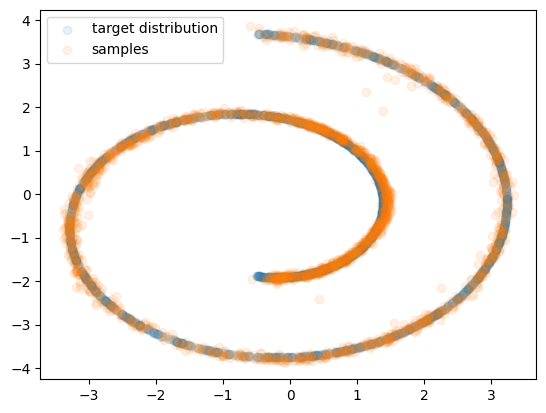
\includegraphics[width=\linewidth]{assets/task1_1/ddpm_samples.png}
    \caption{DDPM, 1000 steps. Chamfer distance $9.41$.}
    \label{fig:swiss_ddpm}
\end{subfigure}
\hfill
\begin{subfigure}[b]{0.48\linewidth}
    \centering
    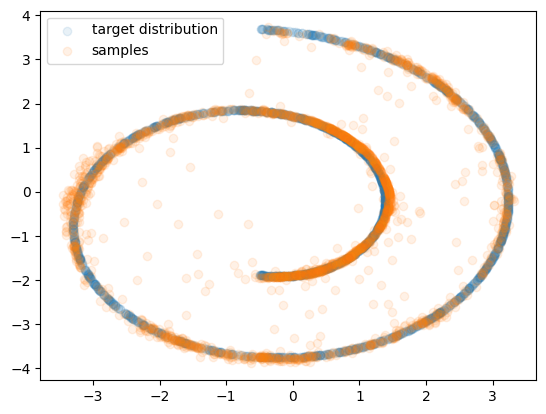
\includegraphics[width=\linewidth]{assets/task1_1/ddim_samples.png}
    \caption{DDIM, 50 steps, $\eta=0$. Chamfer distance $39.78$.}
    \label{fig:swiss_ddim}
\end{subfigure}
\caption{2048 generated samples (orange) against the target Swiss Roll (blue), using the same
network trained for 5000 iterations.}
\label{fig:swiss}
\end{figure}

Both samplers recover the Swiss Roll: the outer sweep and the inner arm are covered, the two arms
stay separated, and there is no mode collapse. The difference is in the outliers. DDPM leaves only a
handful of points off the manifold. DDIM places most points on the spiral too, but a noticeable
scatter of points lies in the empty space between the arms. Since the Chamfer distance sums
nearest-neighbour distances over all points, these outliers are what raise it from $9.41$ to
$39.78$.

This gap is expected for this setting. The network is a small MLP trained for only 5000 iterations,
so its noise prediction has a visible error (Lab 1 showed the loss plateauing around $0.3$). DDPM
takes 1000 small steps and injects fresh noise at each of them, so an error made at one step is
partly washed out by later steps. DDIM with $\eta=0$ takes 50 jumps of 20 timesteps each, with no
noise: each jump commits fully to the current $\hat{\mathbf{x}}_0$, and a point that is pushed in
the wrong direction early has no mechanism to return to the manifold. The result is the same shape at
$20\times$ fewer network evaluations, in exchange for more off-manifold samples.

\subsection{Chamfer Distance}

\begin{figure}[H]
\centering
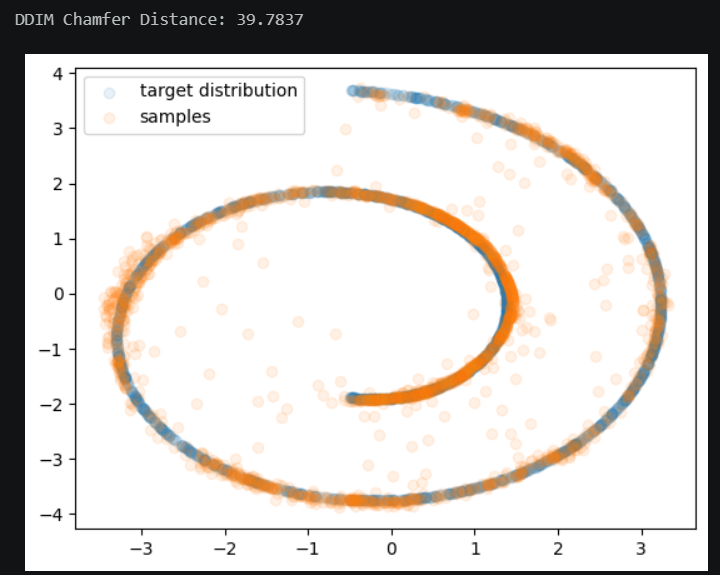
\includegraphics[width=0.6\linewidth]{assets/task1_1/Chamfer_Distance.png}
\caption{Screenshot of the notebook output: DDIM Chamfer distance $= 39.7837$, below the
threshold of $40$.}
\label{fig:cd_screenshot}
\end{figure}


\section{Task 1-2 - DDIM for Image Generation}

For this task I reuse my best checkpoint from Lab 1: the UNet trained on AFHQ $64\times64$ with the
\textbf{linear} beta schedule and the \textbf{noise} predictor for 100k iterations, which reached an
FID of $8.29$ with 1000-step DDPM sampling. The DDPM code (\texttt{add\_noise}, cosine schedule,
predictors and losses) is carried over from Lab 1; only \texttt{DDIMScheduler} is new.

\subsection{Implementation details}
\label{sec:task12_impl}

\subsubsection{TODO \#1 - set\_inference\_timesteps}

\begin{code}
\captionof{listing}{\textbf{DDIM inference schedule}}
\label{code:set_ts}
\begin{minted}
self.num_inference_timesteps = num_inference_timesteps
# Evenly spaced sub-sequence tau_1 < ... < tau_S of {0, ..., T-1}, e.g.
# S=50, T=1000 -> step_ratio=20 and tau = [980, 960, ..., 20, 0].
step_ratio = self.num_train_timesteps // num_inference_timesteps
timesteps = (np.arange(0, num_inference_timesteps) * step_ratio).round()[::-1]
self.timesteps = torch.from_numpy(timesteps.copy().astype(np.int64))
self._ddim_step_ratio = step_ratio
\end{minted}
\end{code}

The inference schedule is an evenly spaced subset of the training timesteps
$\{0,\dots,T-1\}$, stored in descending order because \texttt{model.sample} iterates over
\texttt{self.timesteps} directly. This is the same ``linear'' sub-sequence as in Task 1-1, and the
DDIM paper uses it for its main results. For the step counts in this lab:

\begin{table}[H]
\centering
\caption{Inference timesteps produced for each $S$ ($T=1000$).}
\label{tab:ddim_ts}
\begin{tabular}{rrl}
\toprule
$S$ & \texttt{step\_ratio} & $\tau$ (descending) \\
\midrule
10   & 100 & $900, 800, \dots, 100, 0$ \\
20   & 50  & $950, 900, \dots, 50, 0$ \\
50   & 20  & $980, 960, \dots, 20, 0$ \\
100  & 10  & $990, 980, \dots, 10, 0$ \\
1000 & 1   & $999, 998, \dots, 1, 0$ (the full DDPM chain) \\
\bottomrule
\end{tabular}
\end{table}

Two implementation details. Reversing with \texttt{[::-1]} gives a NumPy array with a negative
stride, which PyTorch cannot wrap directly, so \texttt{.copy()} is required before the
conversion. And \texttt{step\_ratio} is cached as \texttt{\_ddim\_step\_ratio}, because
\texttt{step()} only receives the current $t$ and must recover the previous timestep as
$t - \texttt{step\_ratio}$.

Note that the first inference timestep is $900$ for $S=10$, not $999$. Sampling still starts from
$\mathcal{N}(\mathbf{0},\mathbf{I})$; under the linear schedule $\ab_{900}\approx 3\times10^{-4}$, so
$\mathbf{x}_{900}$ is already pure noise for practical purposes and this mismatch is negligible.

\subsubsection{TODO \#2 - step}

\begin{code}
\captionof{listing}{\textbf{One DDIM step in image space}}
\label{code:ddim_step}
\begin{minted}
if isinstance(t, int):
    t = torch.tensor([t])
t = t.reshape(-1).to(x_t.device)
t_prev = t - self._ddim_step_ratio

# 1. alpha_bar at the current and previous inference timesteps;
#    past the last step (t_prev < 0) alpha_bar_prev = 1, i.e. the clean sample.
alpha_bar_t = extract(self.alphas_cumprod, t, x_t)
alpha_bar_prev = extract(self.alphas_cumprod, t_prev.clamp(min=0), x_t)
is_last = (t_prev < 0).reshape(-1, *([1] * (x_t.ndim - 1)))
alpha_bar_prev = torch.where(is_last, torch.ones_like(alpha_bar_prev), alpha_bar_prev)

# 2. Predicted clean sample, clamped to the image range.
x0_pred = (x_t - (1 - alpha_bar_t).sqrt() * eps_theta) / alpha_bar_t.sqrt()
x0_pred = x0_pred.clamp(-1, 1)

# 3. sigma_t(eta)  (DDIM Eq. 16)
sigma = (
    self.eta
    * ((1 - alpha_bar_prev) / (1 - alpha_bar_t)).sqrt()
    * (1 - alpha_bar_t / alpha_bar_prev).sqrt()
)

# 4. Direction pointing to x_t.
dir_xt = (1 - alpha_bar_prev - sigma**2).clamp(min=0).sqrt() * eps_theta

# 5. x_{t_prev} = sqrt(a_prev) x0_pred + dir_xt + sigma z  (DDIM Eq. 12)
noise = torch.randn_like(x_t)
sample_prev = alpha_bar_prev.sqrt() * x0_pred + dir_xt + sigma * noise
\end{minted}
\end{code}

The math is the same as in Task 1-1 (\autoref{eq:ddim_step}), but three things change in the
batched image setting.

\textbf{Normalizing $t$.} \texttt{model.sample} passes the timestep as a 0-dim tensor taken from
\texttt{self.timesteps}, while other callers may pass a Python \texttt{int}. I convert both to a 1-D
tensor on the image's device, so that \texttt{extract} can gather one $\ab$ per batch element and
reshape it to $(B,1,1,1)$.

\textbf{$\ab_{\tau_{i-1}}$ at the last step, without branching.} In Task 1-1 the template used an
\texttt{if t\_prev >= 0}, which only works when $t$ is a scalar. Here I index with
\texttt{t\_prev.clamp(min=0)} to keep the index valid, then use \texttt{torch.where} to overwrite
the entries with $t_{\text{prev}}<0$ by $1$. As explained in Task 1-1, this makes both $\sigma$ and
the direction term vanish, so the final step outputs $\hat{\mathbf{x}}_0$.

\textbf{Clamping $\hat{\mathbf{x}}_0$.} Images are normalized to $[-1,1]$, so the predicted clean
image is clamped to that range, the same as in the Lab 1 DDPM sampler. This matters more for DDIM
than for DDPM: at large $t$, $\hat{\mathbf{x}}_0$ divides by a tiny $\sqrt{\ab_t}$, and with large
jumps the next state is dominated by $\sqrt{\ab_{\tau_{i-1}}}\,\hat{\mathbf{x}}_0$, so an
out-of-range estimate would directly corrupt the trajectory. The direction term still uses the
unclamped $\boldsymbol{\epsilon}_\theta$, which matches the reference \texttt{diffusers}
implementation.

As a consistency check, setting $S=1000$ and $\eta=1$ makes
$\sigma_t^2=\tilde{\beta}_t$ and the update reduces algebraically to the DDPM posterior step from
Lab 1, so this configuration should reproduce DDPM quality. The results below confirm this.

\subsubsection{TODO \#3, \#4 - Sampling and FID evaluation}

For every combination of $S\in\{10,20,50,100,1000\}$ and $\eta\in\{0.0,0.2,0.5,1.0\}$ I ran
\begin{center}
\texttt{python sampling.py --ckpt\_path \{CKPT\} --save\_dir \{DIR\} --sample\_method ddim
--ddim\_steps \{S\} --eta \{ETA\}}
\end{center}
which generates 500 images, and then measured FID against the AFHQ evaluation split prepared by
\texttt{dataset.py}, using \texttt{fid/measure\_fid.py}.

\subsection{Evaluation results}

\begin{table}[H]
\centering
\caption{FID of DDIM sampling (lower is better). Rows: $\eta$; columns: number of sampling steps
$S$. \textbf{Bold}: best $\eta$ for each $S$. For reference, 1000-step DDPM with the same checkpoint
gives $8.29$.}
\label{tab:fid_ddim}
\begin{tabular}{c|ccccc}
\toprule
\diagbox{$\eta$}{$S$} & 10 & 20 & 50 & 100 & 1000 \\
\midrule
0.0 & 34.18 & 21.30 & 13.04 & 9.29 & 24.55 \\
0.2 & 27.80 & 21.87 & 11.07 & 8.32 & 15.37 \\
0.5 & \textbf{25.53} & \textbf{14.61} & \textbf{10.67} & \textbf{7.58} & 8.11 \\
1.0 & 41.94 & 25.37 & 11.84 & 11.54 & \textbf{7.20} \\
\bottomrule
\end{tabular}
\end{table}

\begin{figure}[H]
\centering
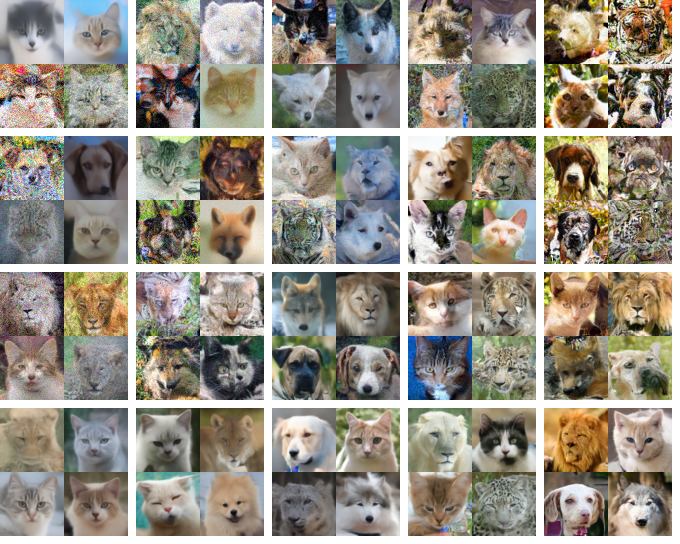
\includegraphics[width=0.9\linewidth]{assets/task1_2/ddim_samples_grid.png}
\caption{Four samples for each setting, laid out like \autoref{tab:fid_ddim}: rows are
$\eta = 0.0, 0.2, 0.5, 1.0$ from top to bottom, columns are $S = 10, 20, 50, 100, 1000$ from left to
right.}
\label{fig:ddim_grid}
\end{figure}

\subsection{Discussion}

\textbf{More steps help, up to a point.} Reading each row from left to right, FID drops steadily
from $S=10$ to $S=100$ for every $\eta$, e.g.\ $34.18 \rightarrow 9.29$ for $\eta=0$ and
$25.53 \rightarrow 7.58$ for $\eta=0.5$. This is discretization error: each DDIM step assumes that
$\hat{\mathbf{x}}_0$ and $\boldsymbol{\epsilon}_\theta$ stay fixed over the whole jump from
$\tau_i$ to $\tau_{i-1}$. With $S=10$ every jump spans 100 training timesteps, the network's
$\hat{\mathbf{x}}_0$ at $t=900$ is close to a dataset average, and the sampler commits to it. The
first column of \autoref{fig:ddim_grid} shows the result: blurry, low-contrast faces for $\eta=0$
and washed-out ones for $\eta=1$.

\textbf{The main result: $20\times$ less compute with no loss in quality.} With $S=50$, every
$\eta$ already reaches FID $\approx 11$--$13$, and with $S=100$, $\eta=0.5$ reaches $7.58$, which is
\emph{better} than the $8.29$ of the full 1000-step DDPM sampler on the same checkpoint. DDIM thus
delivers DDPM-level quality with $10\times$ fewer network evaluations, without any retraining.

\textbf{$\eta=1,\ S=1000$ reproduces DDPM.} As noted in the implementation section, this
configuration is mathematically the DDPM sampler. Its FID of $7.20$ is close to the $8.29$ I measured
in Lab 1. The difference is within the run-to-run variance of a 500-sample FID, so this mostly
confirms that the DDIM step is implemented correctly.

\textbf{Large $\eta$ is bad at few steps.} At $S=10$, $\eta=1$ is the worst setting ($41.94$). The
injected noise $\sigma_t\mathbf{z}$ is sized for the jump between $\tau_i$ and $\tau_{i-1}$, so with
100-timestep jumps each step adds a large amount of fresh noise, and there are not enough remaining
steps to remove it again. This agrees with the DDIM paper (Table 1), where $\eta=1$ at 10 steps is
also by far the worst entry ($41.07$ on CIFAR-10).

\textbf{$\eta=0$ degrades at $S=1000$.} The most surprising entry is $24.55$ for deterministic DDIM
with 1000 steps, much worse than its own $9.29$ at $S=100$. The top-right cell of
\autoref{fig:ddim_grid} shows why: the samples have excessive high-frequency texture and
oversaturated colour noise. A deterministic sampler follows a single trajectory and has no way to
correct an error once it is made. Every one of the 1000 steps adds a small error from the imperfect
$\boldsymbol{\epsilon}_\theta$ and from the inconsistency introduced by clamping
$\hat{\mathbf{x}}_0$ while reusing the unclamped $\boldsymbol{\epsilon}_\theta$, and these errors
accumulate. Stochastic sampling acts as a corrector: the fresh noise partly erases the accumulated
error, and the next prediction pulls the sample back towards the data manifold. This is why, at
$S=1000$, FID improves monotonically with $\eta$ ($24.55 \rightarrow 15.37 \rightarrow 8.11
\rightarrow 7.20$). With fewer steps there are fewer error-accumulating steps, so $\eta=0$ holds up
much better.

\textbf{Difference from the paper.} The DDIM paper reports that $\eta=0$ is best whenever $S$ is
small. In my table a moderate $\eta=0.5$ is best for every $S \le 100$. A likely reason is that my
checkpoint is a modest UNet trained for only 100k iterations. Its noise prediction is less accurate
than the paper's models, so the error-correcting effect of a small amount of noise outweighs the
discretization advantage of the deterministic path. Each FID is also computed from only 500 samples,
so differences of about $1$ (e.g.\ $10.67$ vs.\ $11.07$ at $S=50$) are within noise. The large
effects discussed above (step count, $\eta=1$ at $S=10$, $\eta=0$ at $S=1000$) are well beyond that
margin.

\textbf{Practical choice.} For this model, $S=100$ with $\eta=0.5$ is the best trade-off: FID
$7.58$ at a tenth of DDPM's sampling cost. If sampling speed matters more, $S=50$ costs one
twentieth and still gives FID around $11$.


\section{Task 2-1 - LoRA on a Specific Style}

\subsection{Method and training setup}

LoRA freezes a pretrained weight matrix $W_0\in\mathbb{R}^{d\times k}$ and learns a low-rank update
\begin{equation}
    W = W_0 + \Delta W = W_0 + \frac{\alpha}{r} BA,\qquad B\in\mathbb{R}^{d\times r},\ A\in\mathbb{R}^{r\times k},\ r\ll\min(d,k).
\end{equation}
$B$ is initialized to zero, so training starts exactly from the pretrained model. In
\texttt{train\_lora.py}, LoRA with rank $r=4$ and $\alpha=r$ is attached to the attention
projections (\texttt{to\_q}, \texttt{to\_k}, \texttt{to\_v}, \texttt{to\_out.0}) of the Stable
Diffusion v1.4 UNet. The VAE and text encoder stay frozen. The model is trained with the usual
noise-prediction loss on the VAE latents.

\begin{table}[H]
\centering
\caption{Training configuration (\texttt{scripts/train\_lora.sh}).}
\label{tab:lora_cfg}
\begin{tabular}{ll}
\toprule
Base model & \texttt{CompVis/stable-diffusion-v1-4} \\
Dataset & \texttt{lambdalabs/naruto-blip-captions} \\
Resolution / random flip & $512\times512$ / yes \\
Batch size & 1 \\
Epochs & 15 (about 18k optimization steps) \\
Learning rate / scheduler & $10^{-4}$, constant, no warm-up \\
LoRA rank & 4 \\
Mixed precision & fp16 \\
Seed & 42 \\
Validation prompt & ``a cute bear'' (4 images after every epoch) \\
\bottomrule
\end{tabular}
\end{table}

I changed only two values from the default script: mixed precision from \texttt{no} to
\texttt{fp16}, to fit training into my GPU memory and time budget, and the number of epochs from
100 to 15. As the validation images in \autoref{fig:val_epochs} show, the style is already fully
learned by then.

\subsection{Dataset}

I use the \textbf{Naruto BLIP captions} dataset, \texttt{lambdalabs/naruto-blip-captions}, published
on the Hugging Face Hub by Lambda Labs (\url{https://huggingface.co/datasets/lambdalabs/naruto-blip-captions}).
It contains 1,221 image--text pairs. The images are screenshots of characters from the anime
\emph{Naruto}, collected from Narutopedia. The captions were generated automatically with the BLIP
image-captioning model. The dataset was originally built to fine-tune Stable Diffusion into a
Naruto-style generator.

The dataset suits style LoRA training for three reasons. The visual style is very consistent across
all images: flat cel shading, clean dark outlines, simple backgrounds and the typical anime eye
design. The images are mostly character portraits, so the style is shown on a single kind of
content. And because the BLIP captions describe the \emph{content} (``a man with dark hair'') but
never mention the style, the model has to learn the style as a property of the images rather than
of a trigger word. As a result, the LoRA applies the Naruto style to any prompt.

\subsection{Training images}

\begin{figure}[H]
\centering

\includegraphics[width=\linewidth]{assets/task2_1/train_grid.png}
\caption{Six training images from the Naruto dataset, with their BLIP captions in
\autoref{tab:naruto_captions}.}
\label{fig:naruto_train}
\end{figure}

\begin{table}[H]
\centering
\caption{Captions of the training images in \autoref{fig:naruto_train}, left to right.}
\label{tab:naruto_captions}
\begin{tabular}{cll}
\toprule
\# & Dataset index & Caption \\
\midrule
1 & 0    & a man with dark hair and brown eyes \\
2 & 100  & a man with a bald hair and a bald face \\
3 & 300  & a woman standing in front of a mountain \\
4 & 600  & an older man in a brown robe and a brown robe \\
5 & 900  & a person with blonde hair and green eyes \\
6 & 1200 & a man with white hair and red eyes \\
\bottomrule
\end{tabular}
\end{table}

The captions are short and sometimes inaccurate (image 2 is ``a bald hair and a bald face'', image 4
repeats ``a brown robe''), which is typical of automatic captioning.

\subsection{Generated images}

\begin{figure}[H]
\centering
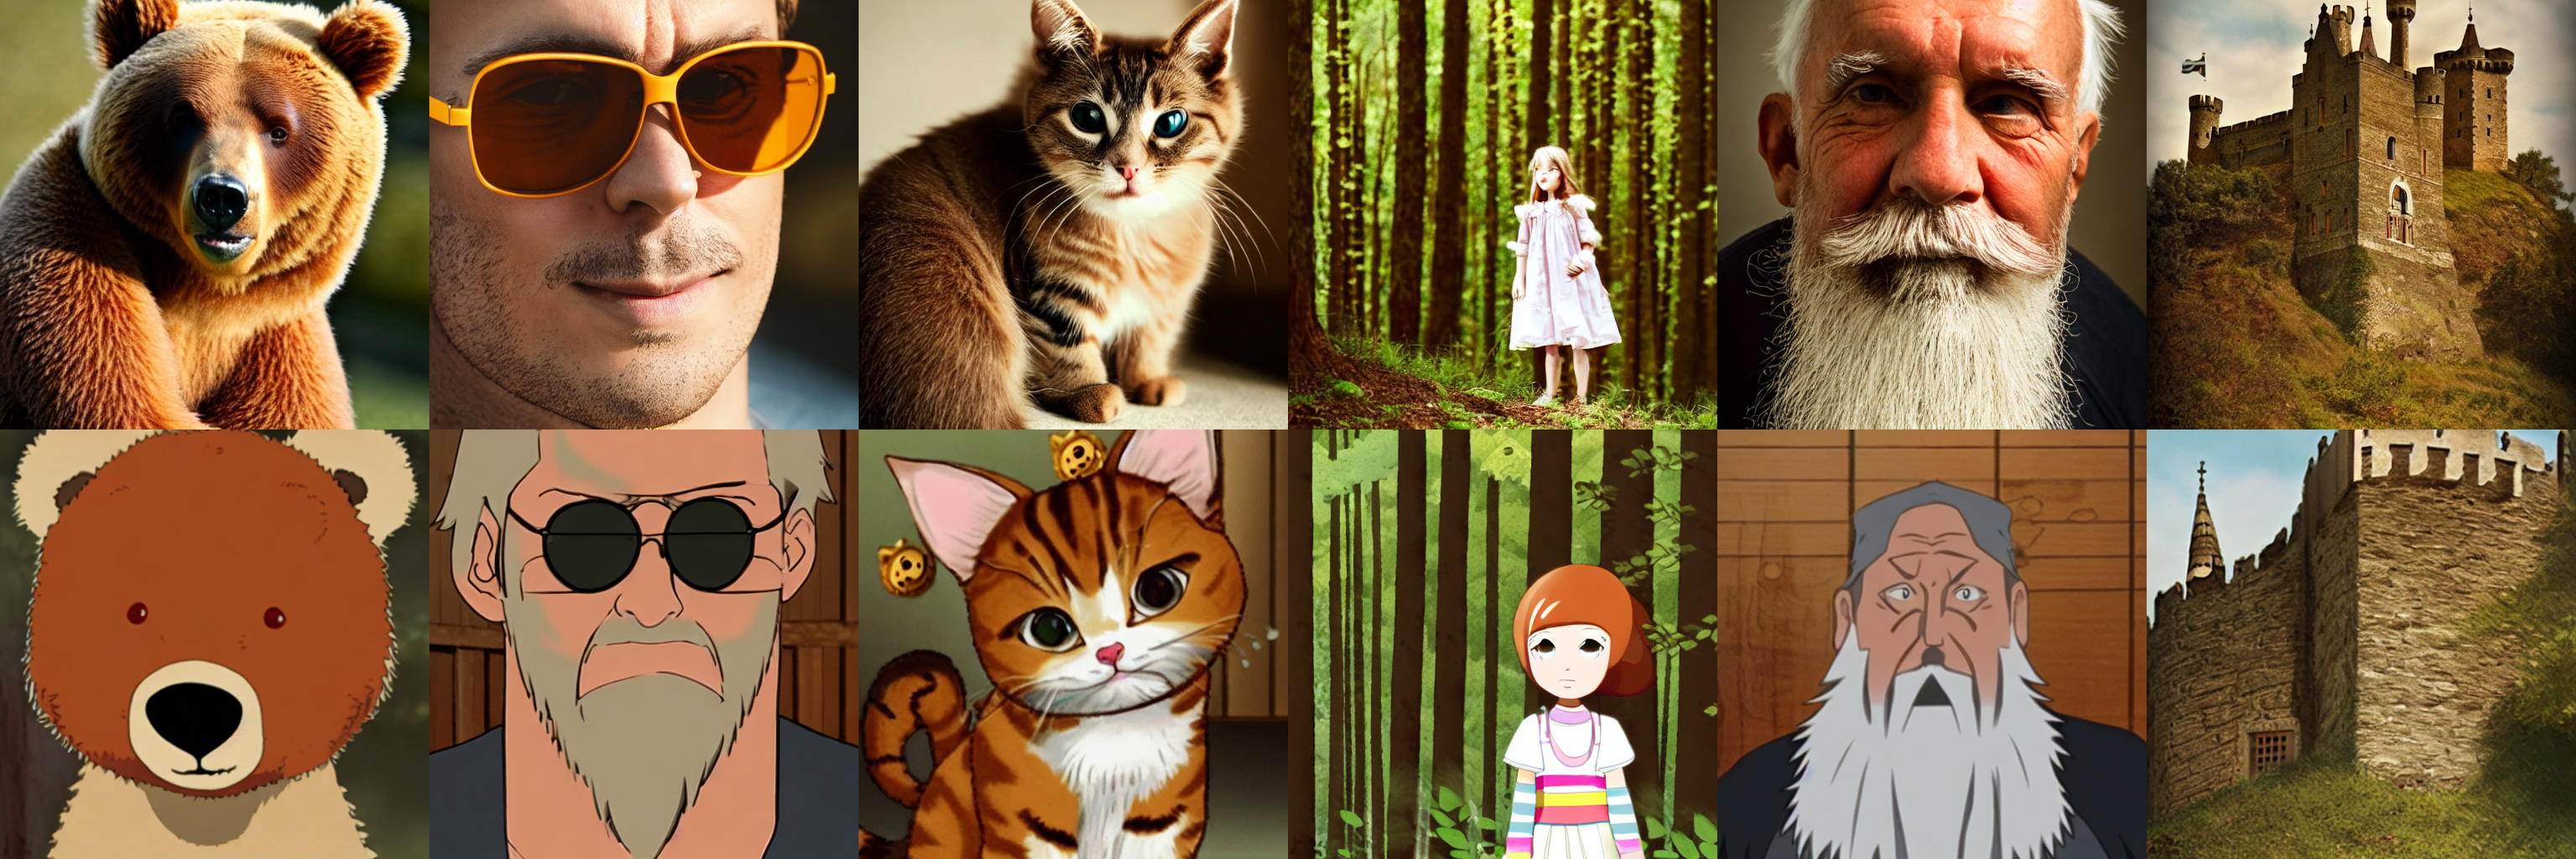
\includegraphics[width=\linewidth]{assets/task2_1/compare_grid.png}
\caption{Top row: base Stable Diffusion v1.4. Bottom row: the same model with the Naruto LoRA.
Each column uses the same prompt and seed. Prompts listed in \autoref{tab:naruto_prompts}.}
\label{fig:naruto_compare}
\end{figure}

\begin{table}[H]
\centering
\caption{Prompts for \autoref{fig:naruto_compare}, left to right. All images: seed 10, 30
inference steps, guidance scale 7.5.}
\label{tab:naruto_prompts}
\begin{tabular}{cl}
\toprule
\# & Prompt \\
\midrule
1 & a cute bear \\
2 & a man with sunglasses \\
3 & a cute cat \\
4 & a girl in a forest \\
5 & an old man with a white beard \\
6 & a castle on a hill \\
\bottomrule
\end{tabular}
\end{table}

None of these prompts mention Naruto or anime, so the base model (top row) produces photographs.
With the LoRA (bottom row) every image switches to the Naruto look, while the content of the prompt
is kept:
\begin{itemize}
    \item \textbf{Characters (2, 4, 5).} Here the style transfer is strongest. The man with sunglasses
    and the old man with a beard are drawn with flat skin tones, thick dark outlines and anime facial
    features. The old man's face strongly resembles the elderly characters in the training set
    (compare training image 4). The girl gets a typical anime face and hairstyle.
    \item \textbf{Animals (1, 3).} The bear and the cat become cartoon characters with flat colour
    fills and simple eyes, even though there are few animals in the training data. The style is
    learned as a rendering style, not tied to human faces.
    \item \textbf{Scenery (6).} The castle shows the weakest effect: it is somewhat flatter and more
    illustrative than the photo, but much less stylized than the characters. This is expected,
    because the dataset contains almost no landscapes or architecture without a character, so the
    LoRA has little evidence about how Naruto draws buildings.
\end{itemize}
The composition stays close to the base model in each column (same pose, framing and colour
palette, e.g.\ the forest in column 4). This is the expected behaviour of a rank-4 update: it changes
\emph{how} things are rendered but keeps most of the base model's knowledge of \emph{what} to
render.

\subsection{Training progress}

\begin{figure}[H]
\centering
\begin{subfigure}[b]{\linewidth}
    \centering
    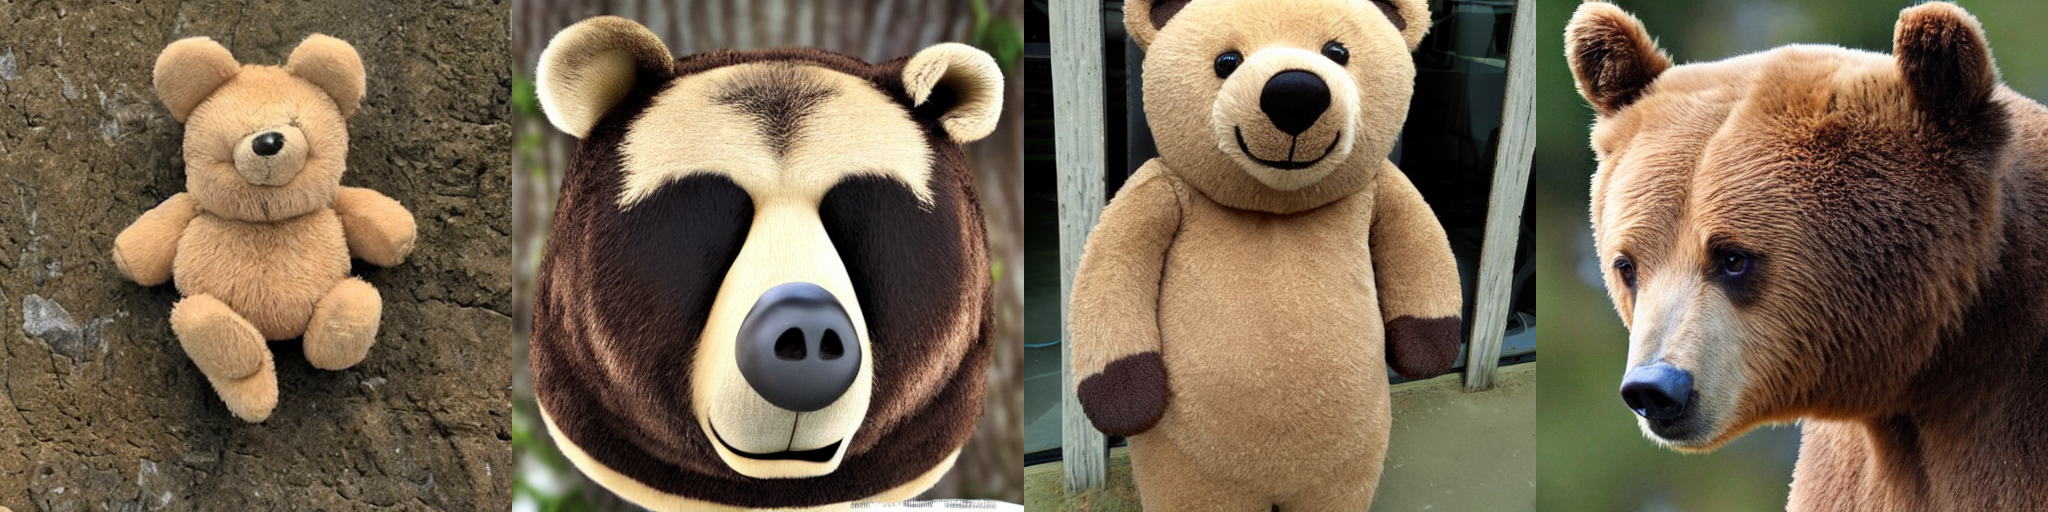
\includegraphics[width=\linewidth]{assets/task2_1/validation_epoch_00.png}
    \caption{After epoch 1}
\end{subfigure}
\\[4pt]
\begin{subfigure}[b]{\linewidth}
    \centering
    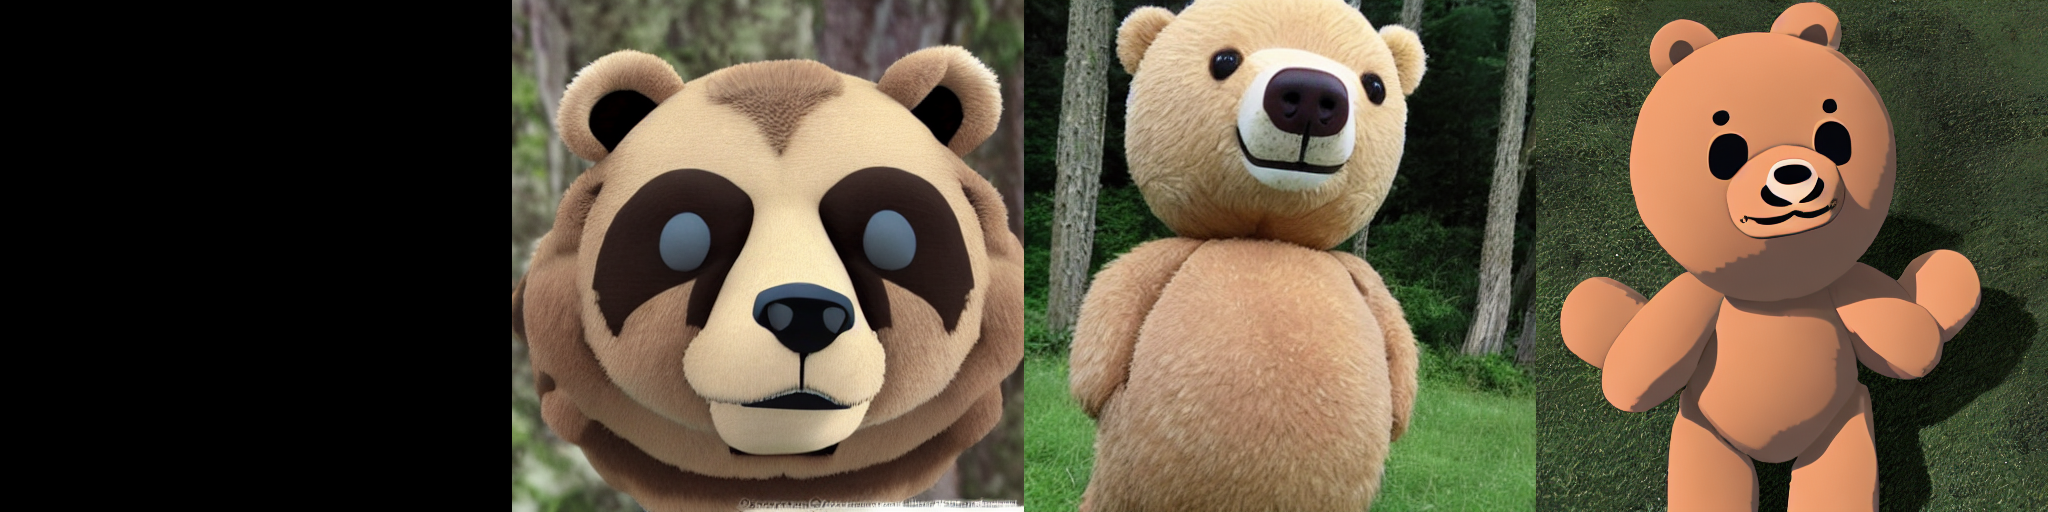
\includegraphics[width=\linewidth]{assets/task2_1/validation_epoch_04.png}
    \caption{After epoch 5}
\end{subfigure}
\\[4pt]
\begin{subfigure}[b]{\linewidth}
    \centering
    
\includegraphics[width=\linewidth]{assets/task2_1/validation_epoch_09.png}
    \caption{After epoch 10}
\end{subfigure}
\\[4pt]
\begin{subfigure}[b]{\linewidth}
    \centering
    
\includegraphics[width=\linewidth]{assets/task2_1/validation_epoch_14.png}
    \caption{After epoch 15 (final)}
\end{subfigure}
\caption{Validation images for the prompt ``a cute bear'' during training.}
\label{fig:val_epochs}
\end{figure}

\autoref{fig:val_epochs} shows how the style is acquired. After the first epoch the outputs are
still photographic (a real bear, teddy bears). By epoch 5 they have become smooth 3D-render-like
plush figures: the photographic texture is gone, but the flat anime look has not arrived yet. From
epoch 10 onward, most samples show flat shading, dark outlines and anime eyes. The black squares at
epochs 5 and 15 are not training failures: they are images that Stable Diffusion's built-in safety
checker flagged (a false positive) and replaced with black.


\section{Task 2-2 - DreamBooth with LoRA on a Specific Identity}

\subsection{Method and training setup}

DreamBooth personalizes a text-to-image model to one specific subject from only a few images. The
idea is to bind the subject to a rare identifier token, here \texttt{sks}, by fine-tuning on the
subject's images with a fixed prompt ``a photo of \texttt{sks} cat''. The class noun ``cat'' lets
the model reuse its prior knowledge of cats, so it only needs to learn what makes \emph{this} cat
different. Combined with LoRA, only the low-rank adapters on the UNet attention layers are trained
(rank 4), so the result is a small weight file instead of a full copy of Stable Diffusion.

\begin{table}[H]
\centering
\caption{Training configuration (\texttt{scripts/train\_dreambooth\_lora.sh}).}
\label{tab:db_cfg}
\begin{tabular}{ll}
\toprule
Base model & \texttt{CompVis/stable-diffusion-v1-4} \\
Instance data & \texttt{task2/sample\_data/dreambooth-cat} (4 images) \\
Instance prompt & ``a photo of \texttt{sks} cat'' \\
Resolution & $512\times512$ \\
Batch size / grad.\ accumulation & 1 / 1 \\
Training steps & 500 \\
Learning rate / scheduler & $10^{-4}$, constant, no warm-up \\
LoRA rank & 4 \\
Mixed precision & fp16 \\
Prior preservation & not used \\
Seed & 0 \\
\bottomrule
\end{tabular}
\end{table}

Compared with the default script I enabled fp16 mixed precision, and I changed the instance prompt
from ``a photo of a \texttt{sks} cat'' to ``a photo of \texttt{sks} cat'', so that \texttt{sks}
directly modifies ``cat'' (the form used in the DreamBooth paper and in my inference prompts).

\subsection{Dataset}

I use the DreamBooth sample dataset provided with the lab template, located in the folder
\texttt{task2/sample\_data/dreambooth-cat}. It contains \textbf{4 images} of the same cat: a fluffy,
long-haired ginger cat with a white chest and muzzle, green eyes and a pink nose. The four images
show the cat sitting or lying in cozy indoor scenes (a living-room floor, a knitted rug, a sofa with
cushions and a window sill) with warm lighting and shallow depth of field. They are close-up shots
with the cat centred and facing the camera.

This is a typical DreamBooth setting: very few images, one subject, and some variation in pose and
background but not in identity. With so few, very similar images, the main risk is overfitting,
where the model learns the backgrounds or lighting along with the cat.

\subsection{Training images}

\begin{figure}[H]
\centering
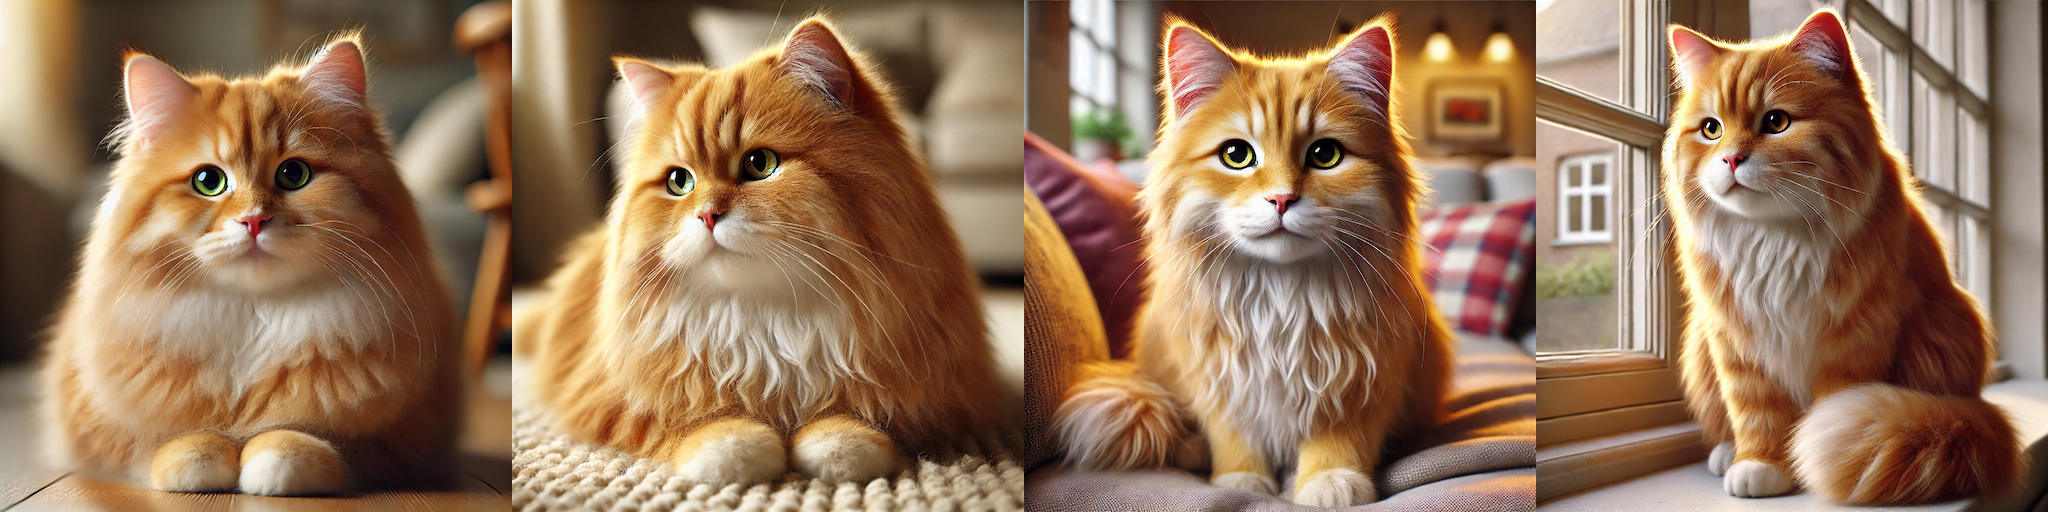
\includegraphics[width=\linewidth]{assets/task2_2/train_grid.png}
\caption{All four training images. Every image is paired with the same instance prompt,
``a photo of \texttt{sks} cat''.}
\label{fig:db_train}
\end{figure}

\subsection{Generated images}

\begin{figure}[H]
\centering
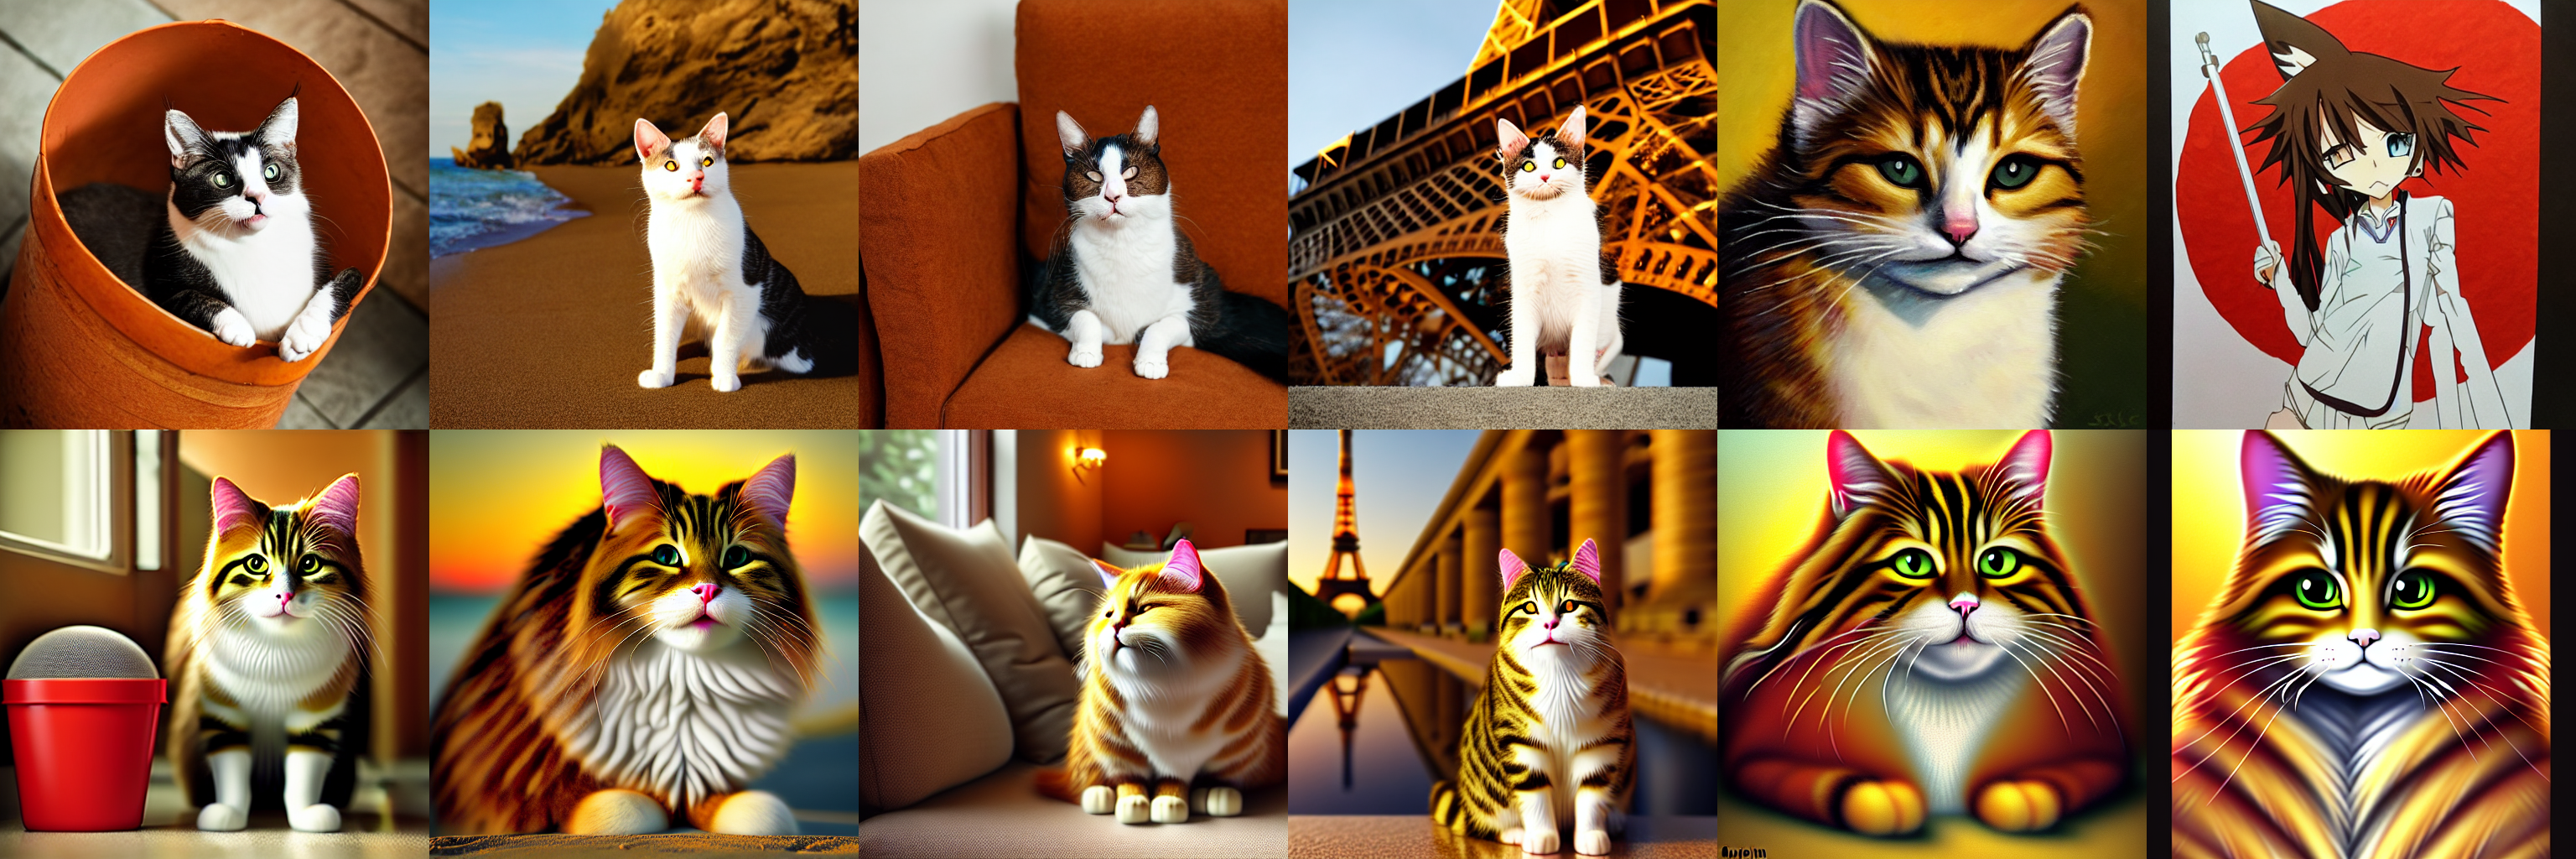
\includegraphics[width=\linewidth]{assets/task2_2/compare_grid.png}
\caption{Top row: base Stable Diffusion v1.4. Bottom row: with the DreamBooth LoRA. Each column uses
the same prompt and seed. Prompts listed in \autoref{tab:db_prompts}.}
\label{fig:db_compare}
\end{figure}

\begin{table}[H]
\centering
\caption{Prompts for \autoref{fig:db_compare}, left to right. All images: seed 10, 30 inference
steps, guidance scale 7.5.}
\label{tab:db_prompts}
\begin{tabular}{cl}
\toprule
\# & Prompt \\
\midrule
1 & A photo of \texttt{sks} cat in a bucket \\
2 & a photo of \texttt{sks} cat on the beach \\
3 & a photo of \texttt{sks} cat sleeping on a sofa \\
4 & a photo of \texttt{sks} cat in front of the Eiffel Tower \\
5 & an oil painting of \texttt{sks} cat \\
6 & an anime drawing of \texttt{sks} cat \\
\bottomrule
\end{tabular}
\end{table}

\textbf{The identity is learned.} For the base model, \texttt{sks} is a meaningless token, so the
top row shows a generic black-and-white cat in each photo, and in column 6 it even draws an anime
girl with cat ears. With the LoRA, every image in the bottom row shows the same kind of cat as the
training set: long fluffy fur, a white chest and muzzle, green eyes and a pink nose, with a ginger
colouring. The identity stays consistent across six very different prompts, and even the anime
prompt now produces the cat instead of a person.

\textbf{The context is followed.} Prompts 2--4 place the cat in new scenes that never appear in
the training data. The beach (2) shows a sunset over the sea, the sofa scene (3) has the cat curled
up with its eyes closed as asked, and in (4) the Eiffel Tower appears in the background. The
oil-painting prompt (5) produces a painterly rendering with visible strokes. So the model can
combine the new identity with its existing knowledge of scenes and styles, which is the purpose of
DreamBooth.

\textbf{Limitations.} The results also show the typical signs of overfitting on four images:
\begin{itemize}
    \item \textbf{Colour bias.} All outputs share the warm orange-yellow palette of the training
    photos, even on the beach and in Paris. The cat is often rendered with stronger tabby stripes and
    more saturated colours than the real one, so the identity is close but not exact.
    \item \textbf{Weaker prompt following.} In (1) the cat sits \emph{next to} a red bucket instead
    of inside it, while the base model places it in the bucket correctly. The identity token pulls
    the image towards the training composition (a cat sitting upright, facing the camera).
    \item \textbf{Style prompts lose strength.} The anime prompt (6) produces a highly saturated
    digital painting rather than an anime drawing, and it looks very similar to the oil painting
    (5). The DreamBooth paper calls this \emph{language drift}: the fine-tuned model starts to
    associate ``\texttt{sks} cat'' with one specific rendering.
\end{itemize}
These issues could be reduced with prior-preservation loss (training on generated images of the
generic class ``a photo of cat'' alongside the instance images), fewer training steps, or more
varied instance images. I did not enable prior preservation in this run.

\end{document}
